\section{Layer 2 Security}

\subsection{Introduction to Secure Communication}

\begin{concept}{Security at Different OSI Layers}\\
Secure communication can be implemented at different layers of the OSI model:
\begin{itemize}
    \item \textbf{Physical Layer (Layer 1)} - Quantum cryptography, physical isolation
    \item \textbf{Data Link Layer (Layer 2)} - IEEE 802.1X, WLAN security (WEP, WPA, WPA2, WPA3), MACsec
    \item \textbf{Network Layer (Layer 3)} - IPsec
    \item \textbf{Transport Layer (Layer 4)} - TLS, QUIC
    \item \textbf{Application Layer (Layer 7)} - PGP, S/MIME, Signal, WhatsApp
\end{itemize}
\end{concept}

\begin{theorem}{Layer Selection Tradeoffs}\\
The choice of which layer to implement security has various tradeoffs:
\begin{itemize}
    \item \textbf{Higher Layer Security}:
    \begin{itemize}
        \item Easier to deploy (often included in applications)
        \item Typically provides end-to-end protection
        \item Less generally applicable (often optimized for specific applications)
    \end{itemize}
    \item \textbf{Lower Layer Security}:
    \begin{itemize}
        \item More difficult to deploy (may require kernel, router, or switch modifications)
        \item Often provides only hop-to-hop protection at layer 2
        \item More generally applicable (protects all protocols above it)
    \end{itemize}
\end{itemize}
\end{theorem}

\subsection{Extensible Authentication Protocol (EAP)}

\begin{definition}{Extensible Authentication Protocol (EAP)}\\
EAP is a framework for authentication that supports multiple authentication methods:
\begin{itemize}
    \item Provides a flexible authentication mechanism
    \item Designed to be transport-independent (can run over various protocols)
    \item Allows network access control without knowledge of each individual user
    \item Supports numerous authentication methods via different EAP types
\end{itemize}
\end{definition}

\begin{code}{EAP Packet Format}\\
EAP packets have a simple structure:
\begin{lstlisting}[language=C, style=basesmol]
struct eap_packet {
    uint8_t code;       // Request (1), Response (2), Success (3), Failure (4)
    uint8_t id;         // Used to match requests and responses
    uint16_t length;    // Total length of the EAP packet
    uint8_t type;       // When code=1,2: authentication method type
    uint8_t data[];     // Type-specific data
};
\end{lstlisting}

Common EAP types include:
\begin{itemize}
    \item Type 4: MD5-Challenge (insecure!)
    \item Type 13: EAP-TLS (recommended)
    \item Type 21: EAP-TTLS
    \item Type 25: PEAP (Protected EAP)
\end{itemize}
\end{code}

\begin{concept}{EAP Authentication Methods}\\
EAP supports numerous authentication methods with varying security properties:
\begin{itemize}
    \item \textbf{EAP-MD5} - Simple challenge-response mechanism (insecure, no mutual authentication)
    \item \textbf{EAP-TLS} - Uses TLS protocol with client certificates (strong security)
    \item \textbf{EAP-TTLS} - Tunneled TLS without requiring client certificates
    \item \textbf{PEAP} - Microsoft's Protected EAP, similar to EAP-TTLS
    \item \textbf{EAP-FAST} - Cisco's Flexible Authentication via Secure Tunneling
\end{itemize}
Current recommendation is to use EAP-TLS when possible.
\end{concept}

\subsection{IEEE 802.1X Port-Based Access Control}

\begin{definition}{IEEE 802.1X}\\
IEEE 802.1X is a standard for port-based network access control:
\begin{itemize}
    \item Controls access to a network by authenticating devices before allowing network access
    \item Prevents unauthorized access through publicly accessible network ports
    \item Uses EAP for authentication
    \item Provides centralized VLAN assignment based on authentication
\end{itemize}
\end{definition}

\begin{concept}{802.1X Components}\\
IEEE 802.1X involves three key components:
\begin{itemize}
    \item \textbf{Supplicant} - The client device requesting network access
    \item \textbf{Authenticator} - The network device (switch, access point) controlling port access
    \item \textbf{Authentication Server} - Typically a RADIUS server that validates user credentials
\end{itemize}
\end{concept}

\begin{KR}{IEEE 802.1X Authentication Process}\\
\paragraph{Initial Connection}
\begin{itemize}
    \item Client connects to a port on the switch/access point
    \item Port is initially blocked for all traffic except EAP
    \item Communication begins with EAPOL (EAP over LAN) protocol
\end{itemize}

\paragraph{Authentication Exchange}
\begin{itemize}
    \item Supplicant sends EAPOL-Start message or authenticator sends EAP-Request Identity
    \item Supplicant responds with identity
    \item Authenticator forwards identity to authentication server using RADIUS
    \item Authentication server and supplicant perform EAP authentication exchange
    \item Authenticator relays EAP messages between supplicant and authentication server
\end{itemize}

\paragraph{Authorization}
\begin{itemize}
    \item Authentication server sends Access-Accept or Access-Reject message
    \item On success, authenticator can include VLAN assignment and other parameters
    \item Authenticator opens port for network access based on authorization parameters
\end{itemize}
\end{KR}

\begin{example}
In an IEEE 802.1X deployment, a user connects their laptop to a corporate network. The switch port is initially closed, blocking all non-authentication traffic. The user's laptop (supplicant) provides credentials through EAP-TLS, and the switch (authenticator) forwards these to a RADIUS server. Upon successful authentication, the RADIUS server instructs the switch to place the user's connection in the appropriate VLAN based on their role. The port is then opened for normal network traffic.
\end{example}

\begin{theorem}{Security Limitations of 802.1X}\\
While 802.1X provides significant security benefits, it has limitations:
\begin{itemize}
    \item Man-in-the-middle attacks are possible when an attacker inserts themselves between a legitimate device and the switch
    \item An attacker could monitor traffic by creating a bridge between the legitimate device and the switch
    \item Once initial authentication is complete, the ongoing session is not continuously verified
    \item These limitations are addressed in 802.1X-2010 with the use of MACsec
\end{itemize}
\end{theorem}

\subsection{MACsec (IEEE 802.1AE)}

\begin{definition}{MACsec}\\
IEEE 802.1AE (Media Access Control Security) provides:
\begin{itemize}
    \item Data confidentiality, integrity, and authenticity on layer 2 (Ethernet)
    \item Protection for all data including DHCP, ARP, and higher layer protocols
    \item Security for both physical and virtual links between devices
    \item Line-rate encryption in hardware implementations
\end{itemize}
\end{definition}

\begin{concept}{MACsec Operation}\\
MACsec operates by:
\begin{itemize}
    \item Encrypting the payload of Ethernet frames between adjacent devices
    \item Adding a SecTAG to identify the keys and provide packet numbering
    \item Adding an Integrity Check Value (ICV) based on GCM-AES
    \item Providing hop-by-hop protection where each device on the path decrypts and re-encrypts the data
\end{itemize}
\end{concept}

\subsection{WLAN Security}

\begin{definition}{WLAN Security Challenges}\\
Wireless networks face unique security challenges:
\begin{itemize}
    \item No physical cable requirement for packet sniffing
    \item Signals extend beyond physical boundaries
    \item Difficult to control who can attempt to connect
    \item Need for strong encryption and authentication
\end{itemize}
\end{definition}

\begin{concept}{Evolution of WLAN Security}\\
WLAN security has evolved through several generations:
\begin{itemize}
    \item \textbf{WEP (Wired Equivalent Privacy)} - Original security standard with major design flaws
    \item \textbf{WPA (Wi-Fi Protected Access)} - Intermediate solution while developing 802.11i
    \item \textbf{WPA2 (IEEE 802.11i)} - Current standard with strong security
    \item \textbf{WPA3} - Newest standard with improved security measures
\end{itemize}
\end{concept}

\subsection{WEP Security}

\begin{definition}{Wired Equivalent Privacy (WEP)}\\
WEP was the original security standard for 802.11 networks:
\begin{itemize}
    \item Shared key between all clients and the access point
    \item Uses RC4 stream cipher with 40 or 104-bit keys
    \item Uses a 24-bit Initialization Vector (IV)
    \item Includes a CRC-32 checksum for integrity checking
\end{itemize}
\end{definition}

\begin{theorem}{WEP Security Flaws}\\
WEP has several critical design flaws:
\begin{itemize}
    \item Small IV space (24 bits) leads to inevitable IV reuse
    \item Weak key scheduling algorithm in RC4
    \item CRC-32 is not cryptographically secure for integrity protection
    \item No protection against bit-flipping attacks
    \item No replay protection
    \item No per-user/per-session keys
\end{itemize}
\end{theorem}

\begin{example}
To demonstrate the weakness of WEP, tools like Aircrack-ng can typically crack a WEP key after capturing approximately one million encrypted frames, a process that takes just minutes to hours depending on network traffic volume. The attack exploits weaknesses in the RC4 key scheduling algorithm, using the predictable IVs to determine key bits.
\end{example}

\subsection{WPA and WPA2}

\begin{definition}{Wi-Fi Protected Access (WPA)}\\
WPA was developed as an interim solution while waiting for 802.11i (WPA2):
\begin{itemize}
    \item Introduced the Temporal Key Integrity Protocol (TKIP)
    \item Provided per-packet key mixing
    \item Added message integrity code (Michael)
    \item Implemented a frame counter to prevent replay attacks
    \item Available in personal (PSK) and enterprise (802.1X) modes
\end{itemize}
\end{definition}

\begin{definition}{WPA2 (IEEE 802.11i)}\\
WPA2 is the complete implementation of the IEEE 802.11i standard:
\begin{itemize}
    \item Introduced Counter Mode with CBC-MAC Protocol (CCMP)
    \item Based on AES encryption (replacing RC4)
    \item Provides stronger authentication, integrity, and confidentiality
    \item Retained TKIP only for backward compatibility
    \item Available in personal (PSK) and enterprise (802.1X) modes
\end{itemize}
\end{definition}

\begin{concept}{WPA/WPA2 Operation}\\
WPA and WPA2 operate in two distinct phases:
\begin{itemize}
    \item \textbf{Authentication Phase}:
    \begin{itemize}
        \item WPA-Personal: Uses pre-shared key (PSK)
        \item WPA-Enterprise: Uses 802.1X and EAP with a RADIUS server
    \end{itemize}
    \item \textbf{Key Exchange Phase}:
    \begin{itemize}
        \item Establishes pairwise transient keys for unicast traffic
        \item Establishes group keys for broadcast/multicast traffic
        \item Implements key rotation to prevent attacks
    \end{itemize}
\end{itemize}
\end{concept}

\subsection{WPA3}

\begin{definition}{WPA3}\\
WPA3 is the latest Wi-Fi security standard (released in 2018):
\begin{itemize}
    \item Introduces Simultaneous Authentication of Equals (SAE) to replace WPA2-Personal PSK
    \item Provides forward secrecy
    \item Protects against offline dictionary attacks
    \item Includes enhanced protection for enterprise networks
    \item Improves encryption for public networks with Opportunistic Wireless Encryption (OWE)
\end{itemize}
\end{definition}

\begin{KR}{Best Practices for WLAN Security}\\
\paragraph{Network Design}
\begin{itemize}
    \item Use WPA2 or WPA3 with CCMP/AES encryption
    \item Implement Enterprise mode with 802.1X authentication when possible
    \item If using Personal mode, use complex pre-shared keys (PSKs)
    \item Use separate SSIDs for different security levels
\end{itemize}

\paragraph{Authentication}
\begin{itemize}
    \item Use EAP-TLS for strongest security
    \item If client certificates aren't feasible, use PEAP or EAP-TTLS
    \item Avoid EAP-MD5 and other weak authentication methods
\end{itemize}

\paragraph{Management}
\begin{itemize}
    \item Change default administrator credentials
    \item Disable unnecessary services like WPS
    \item Update firmware regularly
    \item Use a strong encryption passphrase
\end{itemize}
\end{KR}

\begin{examplecode}{TKIP vs CCMP Comparison}\\
\begin{lstlisting}[language=C, style=basesmol]
// TKIP (Temporal Key Integrity Protocol)
process_with_tkip(packet, key) {
    // For each packet:
    per_packet_key = mix_key(key, IV, MAC_address);  // Key mixing function
    // Use RC4 for encryption
    encrypted_data = rc4_encrypt(per_packet_key, data);
    // Calculate Michael MIC for integrity
    mic = michael_algorithm(key, header, data);
    // Output packet with IV, encrypted data, and MIC
    return format_packet(IV, encrypted_data, mic);
}

// CCMP (Counter Mode with CBC-MAC Protocol)
process_with_ccmp(packet, key) {
    // For each packet:
    // Construct nonce from packet number, addresses, and priority
    nonce = construct_nonce(packet_number, addr, priority);
    // Use AES in counter mode for encryption
    encrypted_data = aes_ctr_encrypt(key, nonce, data);
    // Calculate CBC-MAC for authentication/integrity
    mac = aes_cbc_mac(key, header, data);
    // Output packet with packet number, encrypted data, and MAC
    return format_packet(packet_number, encrypted_data, mac);
}
\end{lstlisting}
\end{examplecode}

\section{Secure Communication and Layer 2 Security}

\subsection{Goals}

\begin{definition}{Security Goals}\\
    \begin{itemize}
        \item \textbf{Confidentiality} Only the communication endpoints can read the data
        \item \textbf{Integrity} The endpoints can detect if data was manipulated
        \item \textbf{Authenticity} Masquerading as an endpoint is not possible
    \end{itemize}
\end{definition}

\subsection{Secure communication protocols at different OSI layers}

\begin{concept}{Layer Comparison}\\
    \begin{itemize}
        \item \textbf{Higher Layers} end-to-end, easier to deploy, less general
        \item \textbf{Lower Layers} hop-to-hop, difficult to deploy, more general
    \end{itemize}
\end{concept}

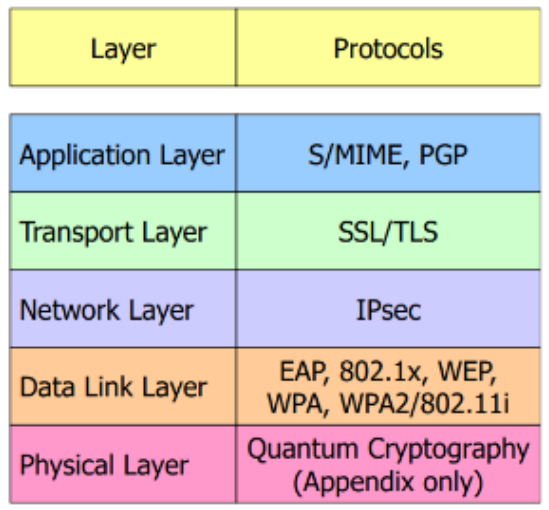
\includegraphics[width=\linewidth]{osi_layers.png}

\subsection{Extensible Authentication Protocol (EAP)}

\begin{definition}{EAP}\\
    Most used standard for L2 authentication
    \begin{itemize}
        \item Supports a wide range of authentication mechanisms
    \end{itemize}
\end{definition}

\subsection{Security of IEEE 802.1x}

\begin{concept}{LAN Access Protection}\\
    Protect access to LANs
    \begin{itemize}
        \item LAN ports are not open per default
        \item Authentication (EAP) is required before accessing a port
        \item Protects against someone plugging in an unauthorized device
        \item Attacker needs access to an authorized physical device
    \end{itemize}
\end{concept}

\subsection{RADIUS (Remote Authentication Dial-In User Service)}

\begin{definition}{RADIUS}\\
    Server / protocol for authentication
\end{definition}

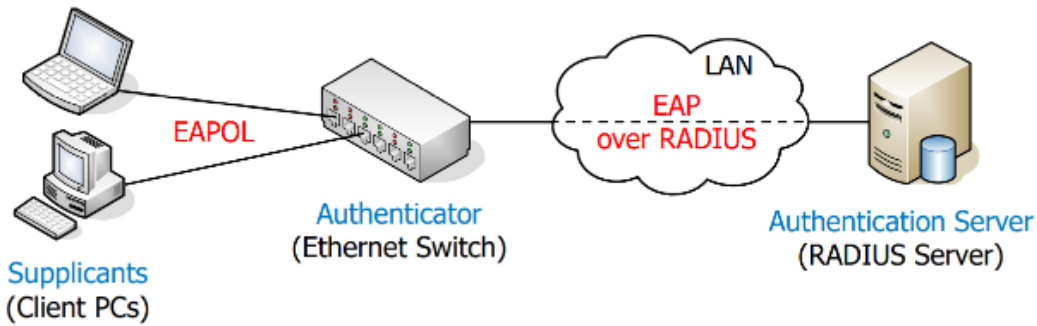
\includegraphics[width=\linewidth]{RADIUS.png}

\subsection{Security mechanisms of WLANs}

\begin{concept}{WLAN Security Needs}\\
    \begin{itemize}
        \item No cable $\rightarrow$ sniffing packets is very easy
        \item Authentication to network is needed
    \end{itemize}
\end{concept}

\subsection{Wired Equivalent Privacy (WEP)}

\begin{definition}{WEP}\\
    \begin{itemize}
        \item All users use the same key long-term
        \item 40- / 104-bit keys (only 104 is good)
        \item 24-bit IV (IV too short $\rightarrow$ repetitions)
    \end{itemize}
\end{definition}

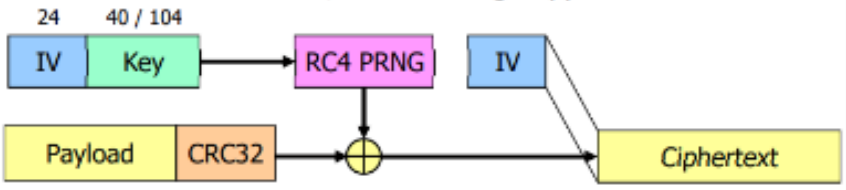
\includegraphics[width=\linewidth]{WEP.png}

\subsection{Wi-Fi Protected Access (WPA) and IEEE 802.11i (WPA2)}

\begin{concept}{WPA/WPA2}\\
    \begin{itemize}
        \item Authentication at Access Point required
        \item Key-Exchange during authentication
        \item WPA: TKIP (default) and CCMP
        \item WPA2: TKIP and CCMP (default)
    \end{itemize}
\end{concept}

\subsection{Temporal Key Integrity Protocol - TKIP}

\begin{definition}{TKIP}\\
    Uses a MAC to protect integrity, however it uses algorithms with well-known weaknesses $\rightarrow$ Insecure
    \begin{itemize}
        \item RC4 (not secure)
    \end{itemize}
\end{definition}

\subsection{Counter Mode CBC-MAC Protocol - CCMP}

\begin{definition}{CCMP}\\
    Uses block cipher to achieve encryption, authenticity, and integrity protection. $\rightarrow$ Considered Secure
    \begin{itemize}
        \item Based on AES (confidentiality and authenticity / integrity)
    \end{itemize}
\end{definition}

% TODO: Add CCMP diagram showing packet processing with AES operations

\subsection{Limits}

\begin{remark}
    \begin{itemize}
        \item Software vulnerabilities, malware, DoS attacks
        \item Protocol design and implementation flaws
        \item Configuration and usability flaws
    \end{itemize}
\end{remark}